\FloatBarrier
\section{Deployment Architecture}

The first version ran only on the developers' laptops. In this phase the system was deployed to the cloud using free tiers of managed services, as shown in Figure~\ref{fig:deploy}. The React application is built into static files and served by Vercel's content delivery network. Vercel also rewrites every \texttt{/api/*} request to the backend, so from the browser's point of view the frontend and the API share one origin and the session cookies are first-party. The backend runs as a Docker container on Render, next to Render's managed Redis, and the database is a managed MySQL~8 service on Aiven, reached over TLS with the provider's CA certificate verified. Behind the rewrite every request passes two proxies (Vercel, then Render), which is why the backend is configured to trust exactly two proxy hops when it reads the client's IP address for rate limiting. Uploaded files live in the database, so the backend container holds no state and can be replaced at any time.

\begin{figure}[H]
\centering
\resizebox{\textwidth}{!}{%
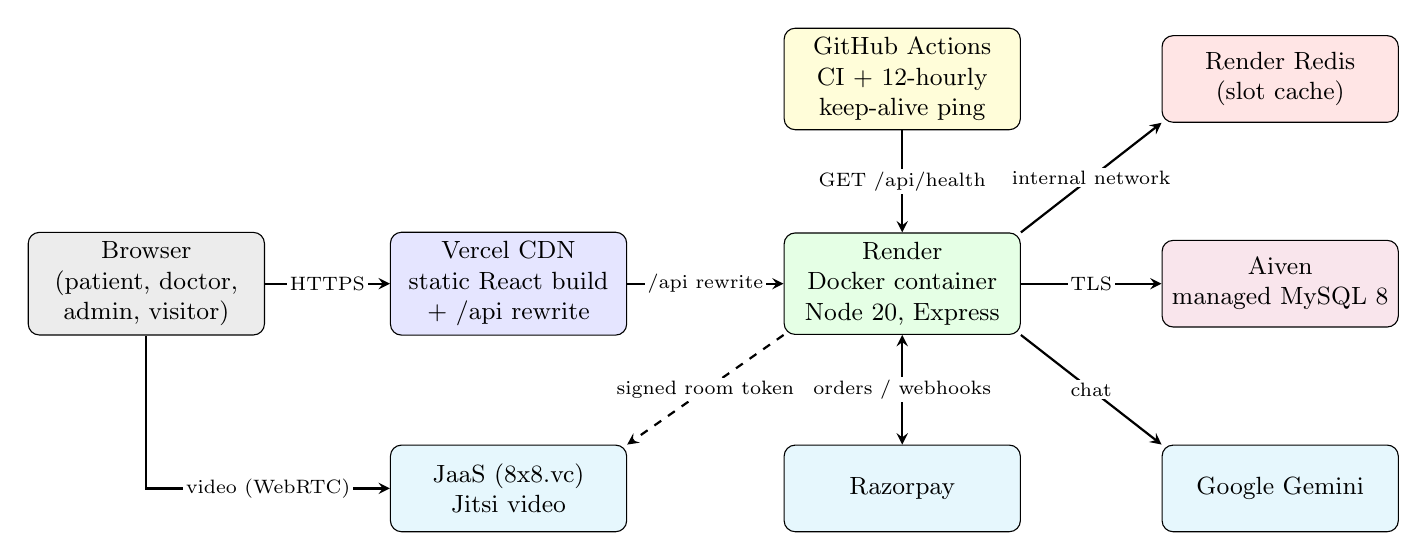
\begin{tikzpicture}[
  box/.style={draw, rounded corners, minimum width=3.0cm, minimum height=1.1cm, align=center, font=\small},
  arr/.style={->, >=stealth, thick},
  lbl/.style={font=\scriptsize, fill=white, inner sep=1pt}
]
\node[box, fill=gray!15] (user) at (0,0) {Browser\\(patient, doctor,\\admin, visitor)};
\node[box, fill=blue!10] (vercel) at (4.6,0) {Vercel CDN\\static React build\\+ /api rewrite};
\node[box, fill=green!10] (render) at (9.6,0) {Render\\Docker container\\Node 20, Express};
\node[box, fill=red!10] (redis) at (14.4,2.6) {Render Redis\\(slot cache)};
\node[box, fill=purple!10] (aiven) at (14.4,0) {Aiven\\managed MySQL 8};
\node[box, fill=cyan!10] (rzp) at (9.6,-2.6) {Razorpay};
\node[box, fill=cyan!10] (gem) at (14.4,-2.6) {Google Gemini};
\node[box, fill=cyan!10] (jit) at (4.6,-2.6) {JaaS (8x8.vc)\\Jitsi video};
\node[box, fill=yellow!15] (gha) at (9.6,2.6) {GitHub Actions\\CI + 12-hourly\\keep-alive ping};
\draw[arr] (user) -- node[lbl]{HTTPS} (vercel);
\draw[arr] (vercel) -- node[lbl]{/api rewrite} (render);
\draw[arr] (render) -- node[lbl]{TLS} (aiven);
\draw[arr, <->] (render) -- node[lbl]{orders / webhooks} (rzp);
\draw[arr] (render.south east) -- node[lbl]{chat} (gem.north west);
\draw[arr] (user.south) |- node[lbl, pos=0.75]{video (WebRTC)} (jit.west);
\draw[arr, dashed] (render.south west) -- node[lbl]{signed room token} (jit.north east);
\draw[arr] (render.north east) -- node[lbl]{internal network} (redis.south west);
\draw[arr] (gha) -- node[lbl]{GET /api/health} (render);
\end{tikzpicture}%
}
\caption{Production Deployment Architecture}
\label{fig:deploy}
\end{figure}

\FloatBarrier
\section{Containerisation}

Both applications have a Dockerfile, and a \texttt{docker-compose.yml} file starts the complete stack locally (MySQL~8, Redis~7, the backend and the frontend served by Nginx) with one command. The backend image is based on \texttt{node:20-alpine}, installs only production dependencies with \texttt{npm ci --omit=dev} (in a separate layer so that it is cached), installs time-zone data, sets \texttt{TZ=Asia/Kolkata}, and runs \texttt{start.sh}. The image needs no volume: prescription files and doctor photos are stored in MySQL, because Render's free plan wipes the container's disk on every restart. Nginx (local stack) and Vercel (production) add the same security headers to the frontend that the API sets on its responses. The CI pipeline builds both images on every change, which guarantees that they always build.

\FloatBarrier
\section{Database Migrations on Start-up}

Render's free plan offers no shell for running one-off commands, so migrations are applied automatically. On every start, \texttt{start.sh} runs the migration script, which applies \texttt{schema.sql} and every migration file through the idempotent runner described in Chapter~\ref{ch:impl}, and then starts the server. A failed migration is logged but does not stop the server: if the database is briefly unreachable at boot, the API still starts, reports \texttt{database: "disconnected"} from its health endpoint, and recovers once the database is back, instead of crash-looping.

\FloatBarrier
\section{Configuration and Secrets}

All configuration is supplied through environment variables, and no secret is committed to the repository. Table~\ref{tab:env} lists the main variables. The Render blueprint (\texttt{render.yaml}) declares them with \texttt{sync: false} so that their values are entered in the dashboard. A separate \texttt{.env.test} file configures the test database, so tests can never touch development or production data.

\begin{longtable}{|L{5.3cm}|L{8.3cm}|}
\caption{Main Environment Variables} \label{tab:env} \\
\hline
\rowcolor{blue!12}
\textbf{Variable} & \textbf{Purpose} \\
\hline
\endfirsthead
\hline
\textbf{Variable} & \textbf{Purpose} \\
\hline
\endhead
NODE\_ENV & \texttt{production} enables Secure/SameSite=None cookies and hides error details \\
\hline
PORT & HTTP port (5001 by default in development) \\
\hline
DB\_HOST, DB\_PORT, DB\_USER, DB\_PASSWORD, DB\_NAME & Database connection \\
\hline
DB\_SSL, DB\_CA\_CERT & TLS to the managed database and the provider's CA certificate for verification \\
\hline
JWT\_SECRET, JWT\_REFRESH\_SECRET & Signing keys for access and refresh tokens \\
\hline
ACCESS\_TOKEN\_TTL\_MIN, REFRESH\_TOKEN\_TTL\_DAYS & Token lifetimes (15 minutes and 7 days by default) \\
\hline
CORS\_ORIGIN & Allowed frontend origin for credentialed CORS requests \\
\hline
GEMINI\_API\_KEY & MediBot \\
\hline
REDIS\_HOST, REDIS\_PORT, REDIS\_PASSWORD & Optional cache; the system works without it \\
\hline
TZ & Must be \texttt{Asia/Kolkata} (Section~\ref{sec:tz}) \\
\hline
TRUST\_PROXY\_HOPS & Proxies in front of the API (default 1; 2 on Render behind Vercel) \\
\hline
RAZORPAY\_KEY\_ID, RAZORPAY\_KEY\_SECRET, RAZORPAY\_WEBHOOK\_SECRET & Payment gateway and webhook verification \\
\hline
PAYMENT\_MODE & \texttt{mock} explicitly allows the mock gateway outside development \\
\hline
JAAS\_APP\_ID, JAAS\_KID, JAAS\_PRIVATE\_KEY & JaaS application, API key id and private key used to sign room tokens \\
\hline
JITSI\_DOMAIN & Jitsi server used when the JaaS keys are empty (default \texttt{meet.jit.si}, which no longer allows embedding; local testing only) \\
\hline
\end{longtable}

\FloatBarrier
\section{Time Zone Handling}
\label{sec:tz}

Appointment slots are stored as a \texttt{DATE} and a \texttt{TIME} column in Indian Standard Time, and many queries compare them with \texttt{NOW()} (for example the join window and the past-appointment check). Cloud servers, however, usually run in UTC. If the Node.js process and the MySQL session used different zones, ``now'' would be 5.5 hours off and patients could be refused, or allowed, at the wrong times. The system therefore sets the zone consistently in three places: the Docker image sets \texttt{TZ=Asia/Kolkata} for the Node.js process, every pooled MySQL connection runs \texttt{SET time\_zone = '+05:30'} before any other query (the offset form needs no time-zone tables on the server), and date arithmetic that must not drift, such as blood expiry dates, is done in UTC on plain date strings. Integration tests create appointments relative to the database's own \texttt{NOW()} so that they behave the same on any machine.

\FloatBarrier
\section{Health Check and Keep-Alive}

\texttt{GET /api/health} returns the API status together with the result of a real database query. Render uses it as the container health check. Aiven's free MySQL tier powers off after about a day without queries, so a scheduled GitHub Actions workflow calls the health endpoint every 12 hours, which both keeps the database active and fails loudly if the deployment is down.

\FloatBarrier
\section{Demonstration Data}

For demonstrations and evaluation, the command \texttt{npm run db:seed-demo} fills the database so that the system looks as it would after some months of use, while respecting every rule of the application. Using the doctors already in the database, it adds 60 patients, two months of past appointments with prescriptions, ratings, payments and cancellations, bookings for the next ten days, blood donors, stock and requests, extra wards with admitted patients, pending bed and discharge requests, and an active emergency board. A second step gives the existing patients about five months of visits with detailed prescriptions (diagnosis, medicines, advice and follow-up) and attaches a one-page prescription PDF on hospital letterhead to nearly every prescription. The seed runs in one transaction, runs only once (demo patients use the reserved domain \texttt{demo.example.com}), keeps booked slots, booking limits, paid video visits and bed occupancy consistent, and refuses to run with \texttt{NODE\_ENV=production} unless \texttt{--yes} is given.

\FloatBarrier
\section{Production Readiness Checklist}

The deployed system runs with test keys and free-tier services. Table~\ref{tab:readiness} lists what must be done before it is used by a real hospital.

\begin{longtable}{|C{0.7cm}|L{6.0cm}|L{6.8cm}|}
\caption{Production Readiness Checklist} \label{tab:readiness} \\
\hline
\rowcolor{blue!12}
\textbf{No.} & \textbf{Item} & \textbf{Reason} \\
\hline
\endfirsthead
\hline
\textbf{No.} & \textbf{Item} & \textbf{Reason} \\
\hline
\endhead
1 & Switch Razorpay to live keys and subscribe the webhook to \texttt{payment.captured}, \texttt{order.paid} and \texttt{payment.failed} & Payments made after the browser is closed are recorded only through the webhook \\
\hline
2 & Issue refunds through the Razorpay Refunds API & Cancelled paid visits are currently only flagged \texttt{refund\_due}; the refund is made by hand in the dashboard \\
\hline
3 & Set the three \texttt{JAAS\_*} keys (or run a self-hosted Jitsi server) under an agreement suitable for clinical data & Without them video falls back to \texttt{meet.jit.si}, which cannot be embedded and is not meant for clinical use \\
\hline
4 & Change the passwords of, or remove, the default demo accounts that \texttt{schema.sql} creates (password \texttt{password}) & They are public in the repository and recreated on start-up if missing \\
\hline
5 & Check \texttt{bed\_allocations} for duplicate open stays before running the bed migration on an existing database & The new unique keys cannot be created while duplicates exist \\
\hline
6 & Move files from MySQL to object storage (e.g. S3) as their number grows & Keeps the database small; the free Aiven tier has 1~GB \\
\hline
7 & Never run the demo data seed against real data & It adds 60 fictitious patients; with \texttt{NODE\_ENV=production} it refuses to run without \texttt{--yes} \\
\hline
8 & Upgrade from free tiers & Free instances sleep when idle, causing slow first requests \\
\hline
9 & Add monitoring and alerting (metrics, error tracking) & Today there are request logs and a health check only \\
\hline
\end{longtable}
